% \usepackage{graphicx}
% \usepackage{listings}
% \usepackage{xcolor}
% \usepackage{float}  % Add this line to use [H] option for figure placement

\lstdefinestyle{bashstyle}{
  language=bash,
  basicstyle=\small\ttfamily,
  commentstyle=\color{green!40!black},
  keywordstyle=\color{blue},
  % frame=single,
  breaklines=true,
  postbreak=\mbox{\textcolor{red}{$\hookrightarrow$}\space},
}

\section{Installation}

\begin{enumerate}
 \item \textbf{Install ethtool}
    \begin{lstlisting}[style=bashstyle]
      sudo apt install ethtool
    \end{lstlisting}
  \begin{figure}[H]
  \centering
  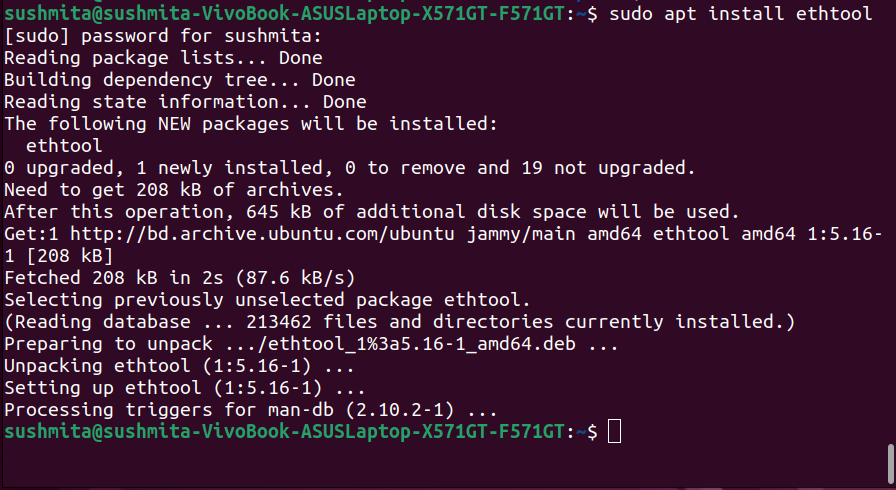
\includegraphics[width=0.8\textwidth]
  {images/install/1_install_ethtool.png}
  \caption{install ethtool}
  \end{figure}
  \item \textbf{Update your system}
    \begin{lstlisting}[style=bashstyle]
      sudo apt-get update
    \end{lstlisting}
    \begin{figure}[H]
    \centering
    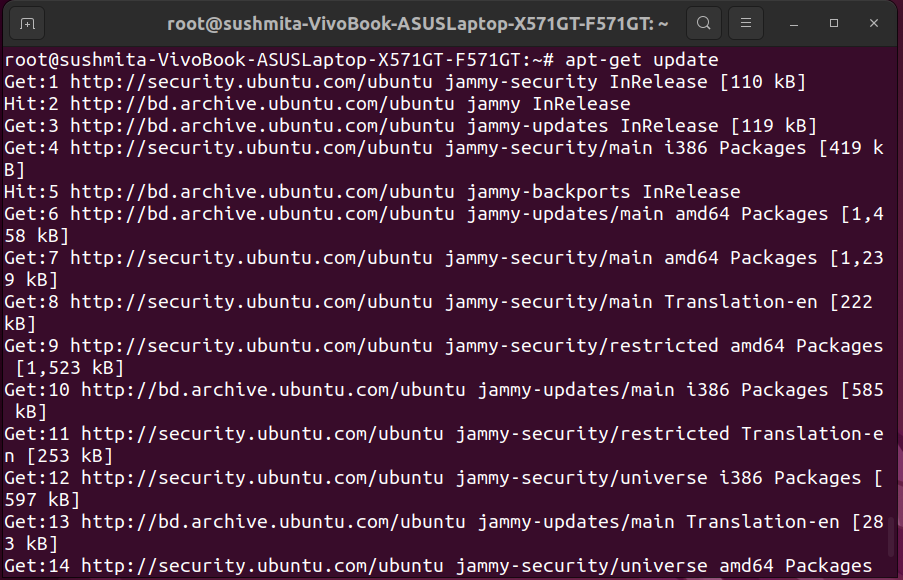
\includegraphics[width=0.8\textwidth]{images/install/2_apt_get_update.png}
    \caption{system update}
\end{figure}
  \item \textbf{Upgrade your system}
    \begin{lstlisting}[style=bashstyle]
      sudo apt-get upgrade
    \end{lstlisting}
    \begin{figure}[H]
  \centering
  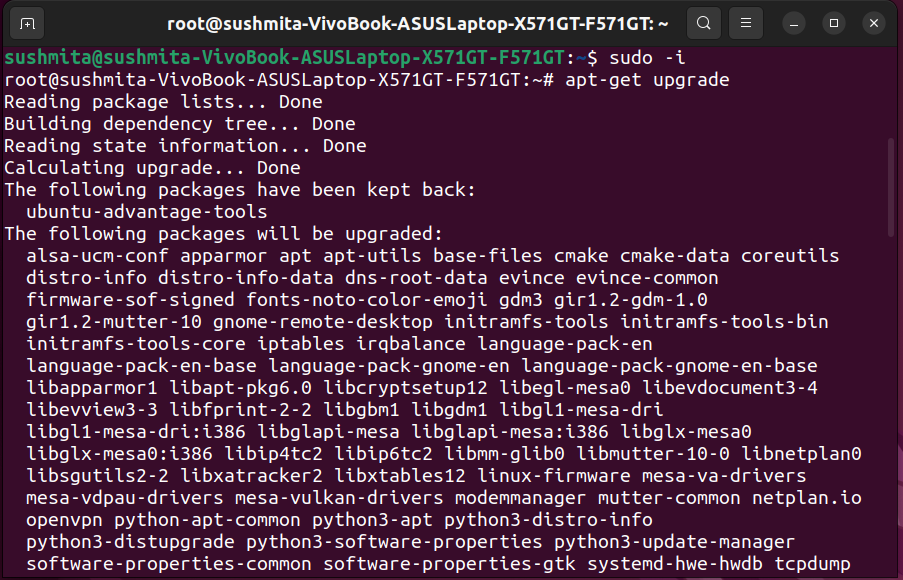
\includegraphics[width=0.8\textwidth]{images/install/3_apt_get_upgrade.png}
  \caption{system upgrade}
\end{figure}
  \item \textbf{Install Zeek pre-req}
    \begin{lstlisting}[style=bashstyle]
      sudo apt-get install cmake make gcc g++ flex bison libpcap-dev libssl-dev python2-dev swig zlib1g-dev
    \end{lstlisting}
    \begin{figure}[H]
  \centering
  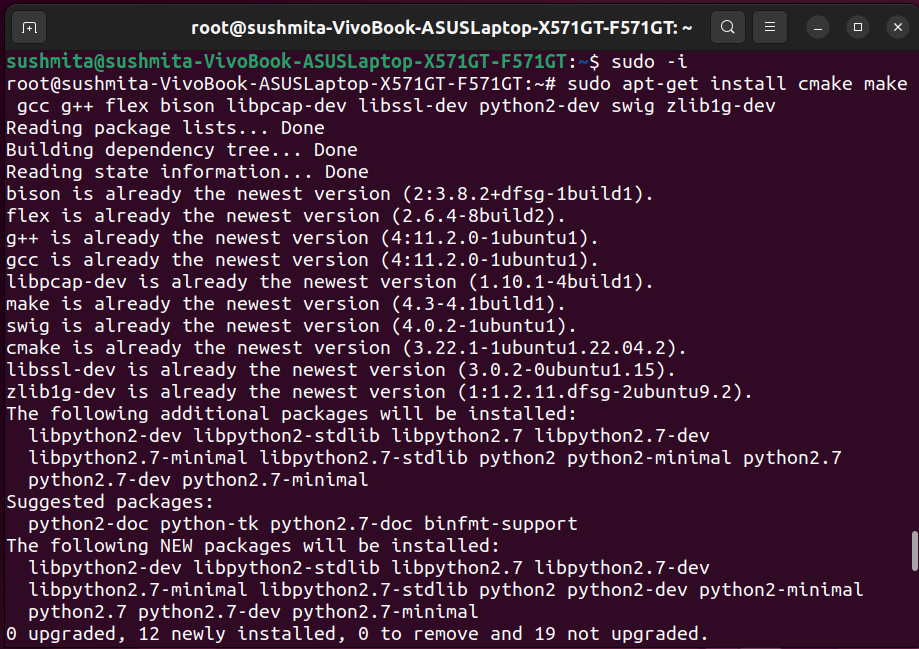
\includegraphics[width=0.8\textwidth]{images/install/4_zeek_prereq_install.png}
  \caption{Zeek pre-req}
\end{figure}
\item \textbf{Check ubuntu version}
    \begin{lstlisting}[style=bashstyle]
      lsb_release -a
    \end{lstlisting}
    \begin{figure}[H]
  \centering
  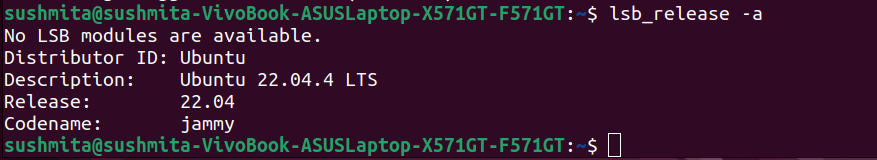
\includegraphics[width=0.8\textwidth]{images/install/5_check_ubuntu_version.png}
  \caption{ubuntu version}
  \end{figure}
  \item \textbf{Add Zeek repositories to local repositories}
    \begin{lstlisting}[style=bashstyle]
      wget -nv https://download.opensuse.org/repositories/security:/zeek/xUbuntu_22.04/Release.key -O Release.key
    \end{lstlisting}
    \begin{figure}[H]
  \centering
  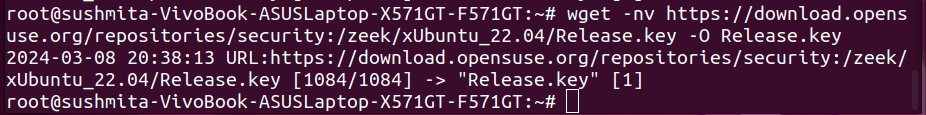
\includegraphics[width=0.8\textwidth]{images/install/6_add_zeek_repo_to_local_repo.png}
  \caption{add zeek repo}
\end{figure}
  \item \textbf{Add key}
    \begin{lstlisting}[style=bashstyle]
      sudo apt-key add -< Release.key
    \end{lstlisting}
    \begin{figure}[H]
  \centering
  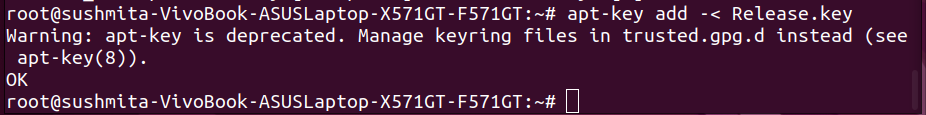
\includegraphics[width=0.8\textwidth]{images/install/7_add_key.png}
  \caption{add key}
\end{figure}
  \item \textbf{Update package to see if there's a new repo}
    \begin{lstlisting}[style=bashstyle]
      sudo apt-get update
    \end{lstlisting}
    \begin{figure}[H]
  \centering
  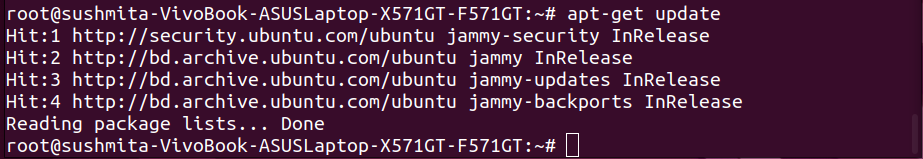
\includegraphics[width=0.8\textwidth]{images/install/8_update_after_addkey.png}
  \caption{update after add key}
\end{figure}
  \item \textbf{Add repo}
    \begin{lstlisting}[style=bashstyle]
      sudo sh -c "echo 'deb http://download.opensuse.org/repositories/security:/zeek/xUbuntu_22.04/ /' > /etc/apt/sources.list.d/security:zeek.list"
    \end{lstlisting}
    \begin{figure}[H]
  \centering
  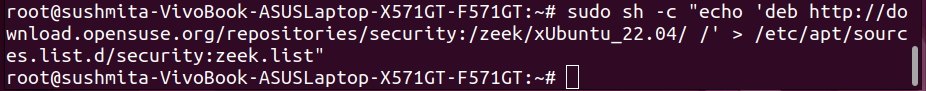
\includegraphics[width=0.8\textwidth]{images/install/9_add_repo.png}
  \caption{add repo}
\end{figure}
  \item \textbf{Update to see if we have any new repo}
    \begin{lstlisting}[style=bashstyle]
      sudo apt-get update
    \end{lstlisting}
    \begin{figure}[H]
  \centering
  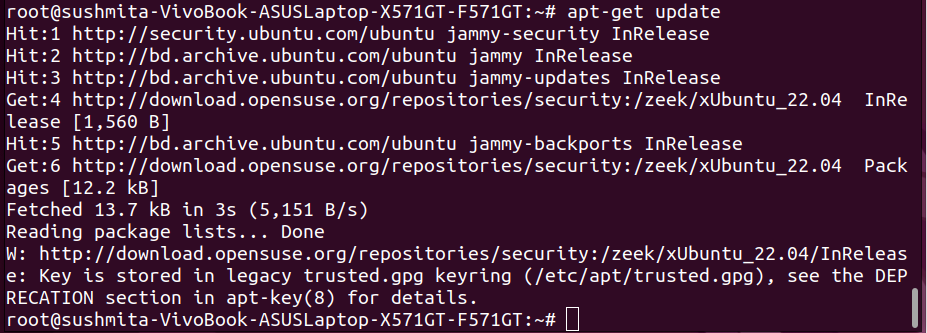
\includegraphics[width=0.8\textwidth]{images/install/10_update_to_see_new_repo.png}
  \caption{update}
\end{figure}
  \item \textbf{Install Zeek}
    \begin{lstlisting}[style=bashstyle]
      sudo apt-get install zeek-lts
    \end{lstlisting}
  \item \textbf{Zeek is now installed!}
  \begin{figure}[H]
  \centering
  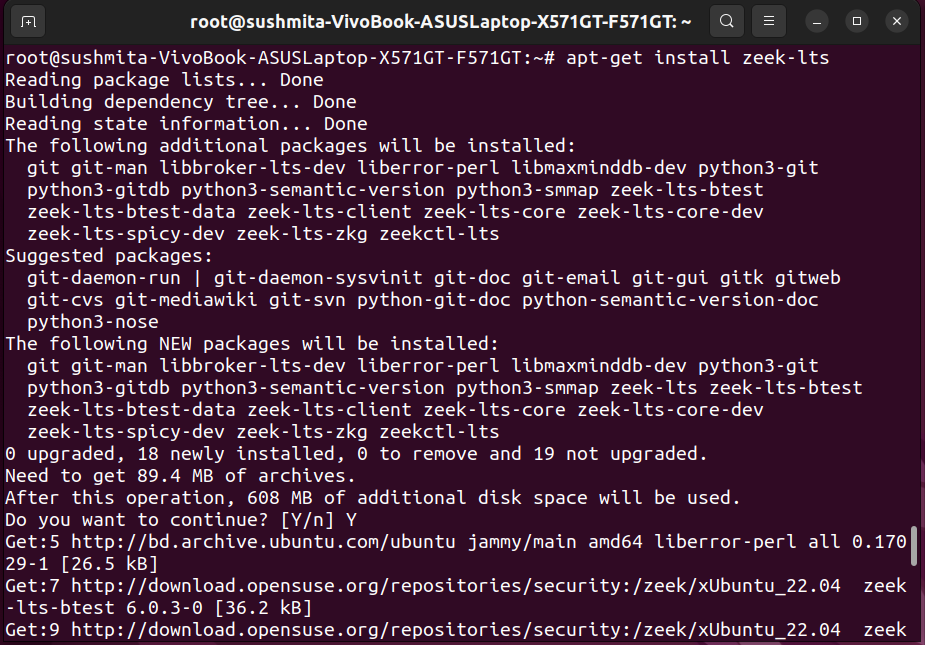
\includegraphics[width=0.8\textwidth]{images/install/11_install_zeek.png}
  \caption{install zeek}
\end{figure}
  \item \textbf{To verify if we have installed}
    \begin{lstlisting}[style=bashstyle]
      ls /opt/
      cd /opt/zeek
      ls
      cd bin/
      ./zeek -h
      ./zeekctl -h
    \end{lstlisting}
  \item \textbf{Installation is verified!}
  \begin{figure}[H]
  \centering
  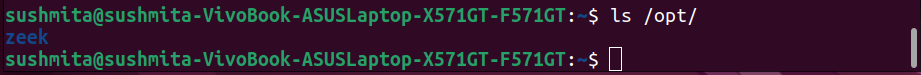
\includegraphics[width=0.8\textwidth]{images/install/12_install_verification.png}
  \caption{Zeek Installation Verification 1}
  \end{figure}
  \begin{figure}[H]
  \centering
  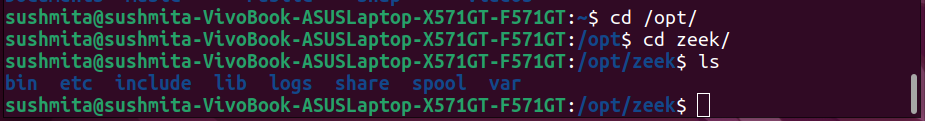
\includegraphics[width=0.8\textwidth]{images/install/13_install_verification.png}
  \caption{Zeek Installation Verification 2}
  \end{figure}
  \begin{figure}[H]
  \centering
  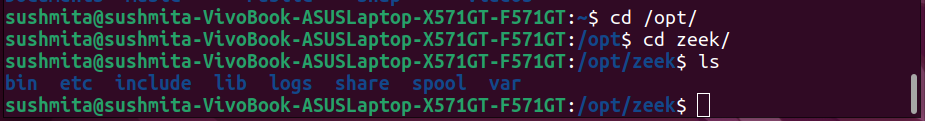
\includegraphics[width=0.8\textwidth]{images/install/13_install_verification.png}
  \caption{Zeek Installation Verification 3}
  \end{figure}
\end{enumerate}
